\chapter{Introduction}

\section{Purpose}
The purpose of 
This chapter serves to set the stage for the relevance of this body of work by exploring some challenges facing computational systems biology and how new web based tools can help.

* Present a toolkit for to make building systems biology web applications easier
* Give a preliminary demonstration at how a new web tool could look like and how it may open new possibilities for a new breed of app

\section{Motivation}

Quantitative analysis and simulation of biological processes are indispensable tools for biomedical research.
Bio-mathematical models have offer the potential to transform the biomedical landscape by revealing the inner workings of biology and enabling virtual experimentation.
Over the past decade, numerous research initiatives, in both the public and private sectors, demonstrate this multidisciplinary field’s growing impact on accelerating drug discovery, developing safer medicine, and improving the understanding of pathogenesis. \autocite{kitano2002computational, kitano2010grand, mack2004can}
Simulation is an indispensable tool in engineering design and has been successfully applied in the automobile, aerospace and telecommunication industries for many years.
Virtual cars are "driven" and virtual aircrafts "flown" under simulated conditions before production and manufacture. \autocite{ghosh2010connecting}
Although the application of advanced modeling techniques has resulted in immense cost savings and standardized protocols for many R\&D-intensive industries, the pharmaceutical industry has historically lacked these approaches, resulting in astronomical drug development costs (25\% of revenues, almost twice that of any other R\&D industry). \autocite{economist2005models}

Systems biology is the natural progression of classical molecular
biology from a descriptive to a quantitative science and is concerned
with the dynamic response of biological networks.

\subsection{Statement Of Problem}

Building models is not an entirely new approach to biology. If one
examines any text book on molecular biology or biochemistry, virtually
every page has a diagram of a model. These models, which are often
termed cartoon based models, represent the culmination of years of
painstaking research; they serve as repositories of accepted doctrine
and the starting point for the generation of new hypotheses. There are,
however, limits to what can be done with these models, their predictive
value tends to be poor, and the ability to reason using qualitative
models is limited. In other sciences these limitations are avoided
through the use of quantitative models, models which are described not
just pictorially but also mathematically. Quantitative models by their
nature have much better predictive value compared to qualitative models,
but their real usefulness stems from the capacity to carry out precise
reasoning with them.
\subsection{What are the advantages of web applications?}

Inherently decoupled, which lends itself to 
However, that is not to say that offline 

problems with deployment
web is the next big platform \autocite{o2007web}
Cisco estimates that the number of devices connected to the Internet will swell from about 10 billion today to 50 billion by 2020 \autocite{clark2014internet}

web is more social \autocite{dabbish2012social}

\subsubsection{The challenge of software deployment and adoption}
challenges with writing cross platform software \autocite{cusumano1999netscape}

\subsubsection{Scientific reproducibility}
\autocite{peng2011reproducible}

\subsubsection{Scalable applications}

\section{Web Applications}

\subsection{A brief history of web applications}
\autocite{w3c2014history}
\autocite{berners2014design}
\begin{itemize}
  \item 1980: Tim Berners-Lee, at CERN, made ENQUIRE a system to use and share documents
  \item 1991: HTML publicly released
  \item 1995: JavaScript written in 10 days by Brendan Eich to be released with Netscape Navigator 2.0
  \item 1996: CSS
  \item 1997: ECMAScript 1
  \item 1998: ECMAScript 2
  \item 1999: ECMAScript 3
  \item 2005: AJAX \autocite{garrett2005ajax}
  \item 2006: jQuery released
  \item 2008: JavaScript the Good Parts 176 pages, JavaScript the Definitive Guide 1100 pages
  \item 2009: Node.js, Angular.js, ECMAScript 5
  \item 2010-today: Backbone, Knockout.js, Ember, Handlebars.js, etc\ldots
\end{itemize}

\subsection{Problem with Web Security}

\autocite{grier2008secure}

\subsection{DOM}

The Document Object Model (DOM) is one of the central conventions in web browsers for representing

\begin{figure}
  \centering
  \includegraphics[width=0.5\textwidth, page=22, trim=0cm 0cm 11cm 0cm, clip=true]{images/Figures.pdf}
  \caption{Hierarchy of objects in a web browser DOM. Like HTML, DOM elements follow a tree structure.}
  \label{Figure:dom}
\end{figure}


\subsection{Single Page Web Applications}

\begin{figure}
  \centering
  \includegraphics[width=\textwidth, page=3]{images/Figures.pdf}
  \caption{How JQuery and Angular scale for complex JavaScript Web Applications.}
  \label{Figure:jquery-vs-angular}
\end{figure}

declarative programming should be used for building user interfaces and wiring software components, while imperative programming is excellent for expressing business logic


Decouple DOM manipulation from application logic. This improves the testability of the code. Regard application testing as equal in importance to application writing. Testing difficulty is dramatically affected by the way the code is structured.
Decouple the client side of an application from the server side. This allows development work to progress in parallel, and allows for reuse of both sides.
Guide developers through the entire journey of building an application: from designing the UI, through writing the business logic, to testing.
Angular follows the MVC pattern of software engineering and encourages loose coupling between presentation, data, and logic components. Using dependency injection, Angular brings traditional server-side services, such as view-dependent controllers, to client-side web applications. Consequently, much of the burden on the backend is reduced, leading to much lighter web applications.

\subsection{HTML5}
\label{sec:html5}

\section{Specific Results}
\subsection{Aim 1 - Chapter~\ref{chap:graphene}: Produce a web library for building interactive and graphical applications}
\subsection{Aim 2 - Chapters~\ref{chap:tidal},~\ref{chap:redox}: Integrate Graphene into new and existing applications}
\subsection{Aim 3 - Chapters~\ref{chap:carbon},~\ref{chap:engine}: Build server-side architecture for modeling applications}


